% -------------------------------------------------------------------------------
% Establish page structure & font.
\documentclass[12pt]{report}

\usepackage[total={6.5in, 9in},
	left=1in,
	right=1in,
	top=1in,
	bottom=1in,]{geometry} % Page structure

\usepackage{graphicx} % Required for inserting images
\graphicspath{{../.images/}} % Any additional images I use (BCU logo, etc) are from here.

\usepackage[utf8]{inputenc} % UTF-8 encoding
\usepackage[T1]{fontenc} % T1 font
\usepackage{float}  % Allows for floats to be positioned using [H], which correctly
                    % positions them relative to their location within my LaTeX code.
\usepackage{subcaption}
% \usepackage[british]{babel}
\usepackage{csquotes}

\usepackage{pdflscape} % Enables the page to be rotated 
                       % landscape for easier image viewing.

% -------------------------------------------------------------------------------
% Declare biblatex with custom Harvard BCU styling for referencing.
\usepackage[
    useprefix=true,
    maxcitenames=3,
    maxbibnames=99,
    style=authoryear,
    dashed=false, 
    natbib=true,
    url=false,
    backend=biber
]{biblatex}

% Additional styling options to ensure Harvard referencing format.
\renewbibmacro*{volume+number+eid}{
    \printfield{volume}
    \setunit*{\addnbspace}
    \printfield{number}
    \setunit{\addcomma\space}
    \printfield{eid}}
\DeclareFieldFormat[article]{number}{\mkbibparens{#1}}

% Declare it as the bibliography source, to be called later via \printbibliography
\addbibresource{litReview.bib}

% -------------------------------------------------------------------------------
% To prevent "Chapter N" display for each chapter
\usepackage[compact]{titlesec}
\usepackage{wasysym}
\usepackage{import}

\titlespacing*{\chapter}{0pt}{-2cm}{0.5cm}
\titleformat{\chapter}[display]
{\normalfont\bfseries}{}{0pt}{\Huge}

% -------------------------------------------------------------------------------
% Custom macro to make an un-numbered footnote.

\newcommand\blfootnote[1]{
    \begingroup
    \renewcommand\thefootnote{}\footnote{#1}
    \addtocounter{footnote}{-1}
    \endgroup
}

% -------------------------------------------------------------------------------
% Fancy headers; used to show my name, BCU logo and current chapter for the page.
\usepackage{fancyhdr}
\usepackage{calc}
\pagestyle{fancy}

\setlength\headheight{37pt} % Set custom header height to fit the image.

\renewcommand{\chaptermark}[1]{%
    \markboth{#1}{}} % Include chapter name.


% Lewis Higgins - ID 22133848           [BCU LOGO]                [CHAPTER NAME]
\lhead{Lewis Higgins - ID 22133848~~~~~~~~~~~~~~~
\includegraphics[width=1.75cm]{BCU}}
\fancyhead[R]{\leftmark}

% ------------------------------------------------------------------------------
% Used to add PDF hyperlinks for figures and the contents page.

\usepackage{hyperref}

\hypersetup{
    colorlinks=true,
    linkcolor=black,
    filecolor=magenta,
    urlcolor=blue,
    citecolor=black,
}

% ------------------------------------------------------------------------------
\usepackage{xcolor} 
\usepackage{colortbl}
\usepackage{longtable}
\usepackage{amssymb}
% ------------------------------------------------------------------------------

% ------------------REMOVE ME --------------------------------------------------

% Temp, using to add notes for the draft edition.
\usepackage{tcolorbox}

% ----------------- REMOVE ME --------------------------------------------------

\begin{document}

    \makeatletter
    \begin{titlepage}
        
\includegraphics[width=0.3\linewidth]{BCUWide.jpg}\\[4ex]
        \vspace{1cm}
        \begin{center}
            {\huge \bfseries  CMP6200}\\[2ex]
            {\huge \bfseries  Individual Undergraduate Project}\\[2ex]
            {\huge \bfseries 2024 - 2025}\\[6ex]
            {\large \bfseries A2 - Literature Review and Methods}\\[10ex]
            {\huge \bfseries University Artifically Intelligent Assistant}\\[6ex]
            
\includegraphics[width=0.1\linewidth]{Symbol.png}\\[40ex]
            Course: Computer \& Data Science\\
            Student Name: Lewis Higgins\\
            Student Number: 22133848\\
            Supervisor Name: Dr. Atif Azad
        \end{center}
    \end{titlepage}
    \makeatother
    \thispagestyle{empty}
    \newpage

    \tableofcontents
    %\footnotesize{\listoffigures}

    \chapter{Report Introduction}\label{ch:introduction}

    \begin{tcolorbox}[colback=orange!5!white,colframe=orange!75!black,title=Draft notice]
        This is a very early draft of this literature review and will be subject to major change
        over the next month. I've marked sections that I've taken from the proposal, or ones that 
        I'm currently uncertain of, with boxes similar to this one.
    \end{tcolorbox}


    \section{Aims and Objectives}

    \begin{tcolorbox}[colback=red!5!white,colframe=red!75!black,title=Copied from proposal]
        These are still subject to change pending the grade from my proposal.
    \end{tcolorbox}

    \noindent
    This project aims to aid new and existing students alike while they are attending university with 
    helpful information about the university itself, such as university societies, locations/campuses, 
    and policies through the medium of a digital chatbot companion to converse with.
    Its objectives are to:

    \begin{itemize}
        \item Develop a chatbot capable of accurately answering user queries related to university 
        buildings, policies, and societies with a minimum 95\% accuracy rate.
        \item Conduct a thorough literature review on the surrounding topics, namely AI, LLMs and NLP.
        \item Create effective documentation for all stages of development, highlighting challenges faced during the process.
        \item Manage time effectively to ensure all project milestones are met on a consistent and regular timeframe.
        \item Evaluate the effectiveness of an AI assistant on university student acclimatization.
    \end{itemize}

    \pagebreak % REMOVE ME IF UNNECESSARY

    \section{Literature Search Methodology}

    \noindent 
    My literature search will be performed using multiple reputable databases for academic papers, including:
    \begin{itemize}
        \item IEEE Xplore
        \item Scopus / Elsevier
        \item Google Scholar
        \item BCU Online Library
    \end{itemize}
    
    \noindent By using multiple different databases to source my information from, I can ensure that
    any potentially relevant literature will be found. Figure \ref{fig:litSearch} depicts 
    how in a search for 1685 articles about employee retention strategies and turnover, only 582 (25.7\%) appeared in multiple databases
    \autocite{litSearch}, meaning that the remaining 74.3\% of articles were exclusive to the single 
    database in which they were found, emphasising the importance of searching multiple databases.  

    \begin{figure}[H]
        \centering
        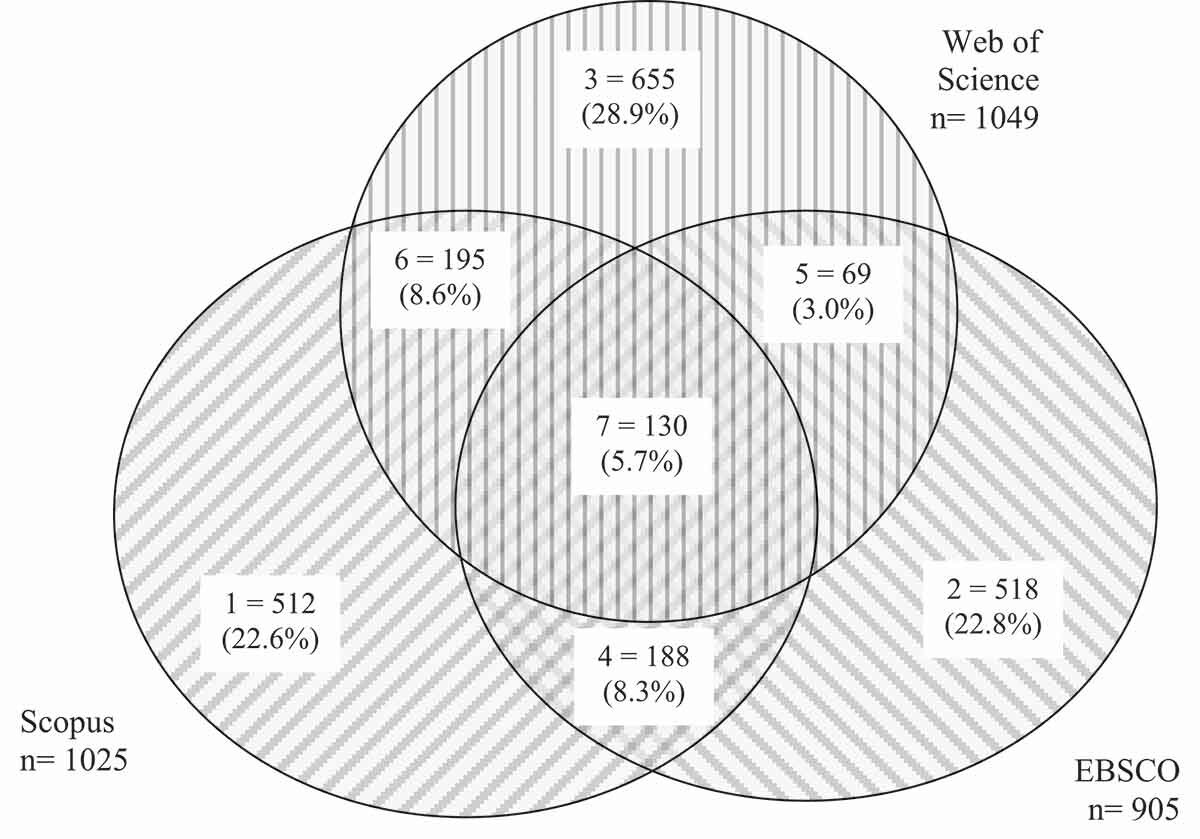
\includegraphics[width=.6\linewidth]{litSearchDBs.jpg}
        \caption{Distribution of searched articles across databases. \autocite{litSearch}}
        \label{fig:litSearch}
    \end{figure}
   
    \noindent 
    All searches performed for recent literature will be on papers published during or after 2017, with a preference 
    to more recent literature, due to the constantly evolving fields my project is based on. 
    The search terms I will use to retrieve the data I will be studying are:

    \begin{itemize}
        \item Artifical Intelligence / AI 
        \item Chatbots / Digital Assistants
        \item Natural Language Processing / NLP
        \item Large Language Models / LLMs
        % \item Human-Computer Interaction
        % \item Knowledge Bases
        % \item Deep learning
        \item User Experience / UX
        % \item Information retrieval
    \end{itemize}

    \noindent
    By using these specific terms that are directly relevant to the core themes of my project,
    I will be ensuring that I only retrieve literature that will be of crucial use in its 
    development.


    \chapter{Literature Review}

    \section{Themes}

    To develop the artefact and conduct thorough background research on relevant literature to further my 
    knowledge of the subject areas, key general themes of the project were identified. From these themes, further 
    keywords to be used in the literature search were derived to ensure that retrieved literature is directly relevant 
    to my research and development of the final artefact. Due to the constantly evolving fields the project focuses 
    on, it will be necessary to limit the results to only those written in recent years (2018 earliest) as there are 
    frequent new developments in the subject areas.

    % \begin{tcolorbox}[colback=red!5!white,colframe=red!75!black,title=Significant uncertainty]
    %     I had a large amount of difficulty identifying my project's key themes, as many of them overlap and I was
    %     unsure which would simply be keywords of others, which is most evident with "AI" and "Generative AI" seen below.
    %     From what I can gather so far, I'm not sure if just making a chatbot that just accesses another LLM's API is worthy 
    %     of being a dissertation project at all, and if it would be better to try with my own fine-tuned model of something 
    %     like LLaMA. I'd have much more to write about that way.
    % \end{tcolorbox}
\pagebreak
    \begin{tcolorbox}[colback=red!5!white,colframe=orange!75!black,title=Uncertainty]
        Chatbots / Digital assistants are highlighted red due to my uncertainty of whether they should 
        be a key theme of the literature review. This is because recent ones use NLP and LLMs, which already have
        their own themes I intend to review.
    \end{tcolorbox}

    \begin{table}[H]
        \centering
        \begin{tabular}{|p{0.2\textwidth}|p{0.52\textwidth} | p{0.23\textwidth}|}
            \hline
            \cellcolor{blue!25}Theme & \cellcolor{blue!25}Description &
            \cellcolor{blue!25}Keywords \\

            \hline

            AI & A field of computing dedicated to allowing computers to simulate human
            learning by training them on large amounts of data so that they can recognise patterns to classify or 
            predict unknown data. AI can only be as good as the data it is trained upon, and can 
            develop biases if it is fed too much data of a certain type. & Generative AI, 
            Human-Centred AI, Explaianble AI, AI Ethics, AI Bias \\

            % \hline

            % Generative AI & AI dedicated to the generation of content rather than prediction or 
            % classification. It is possible for generative AI to produce text, images and 
            % more recently, even video and sound. & LLMs, Tokens, Embedding \\

            \hline
            \cellcolor{red!25} Chatbot \newline Digital Assistant & \cellcolor{red!25} Software that simulates a natural conversation between the 
            computer and end user. Many chatbots, including the one I intend to develop, utilise recent
            developments such as Generative AI and natural language processing (NLP) to interpret and respond to user queries.
            \autocite{IBMChatbotDef}
            & \cellcolor{red!25} NLP, 
            Microsoft Bot Framework, Watson Assistant, ChatGPT \\

            \hline 

            Natural Language Processing & NLP refers to the use of machine learning to encode and 
            process text to understand it in a similar way to humans, which can be used to allow direct 
            two-way conversation between users and computers. & Deep learning, Tokenization, Sentiment analysis,
            Entity linking

            \\

            \hline
            
            LLMs & Large Language Models are a type of AI dedicated to the recognition and generation of text.
            As suggested by their name, they are trained on enormous amounts of text data, which allows them 
            to have active conversations with users. There are many different LLMs, and as their size and 
            complexity increases, so too does the necessary processing power. &
            Retrieval augmented generation (RAG), Fine-tuning, Prompt engineering, 
            GPT4o, LLaMA, Gemini, Claude
            
            \\

            \hline

            User Experience (UX) & The end user's overall experience of using a system, such as its ease of use and 
            whether it is enjoyable to use \autocite{UXDict}. In the context of my project, it will refer to the user's 
            ability to smoothly converse with the chatbot and how human-like it is. 
            & Conversational design, usability, market research, human-computer interaction

            \\

            \hline 

        \end{tabular}\label{tab:themes}
    \end{table}


    \pagebreak % REMOVE IF NECESSARY

    \section{Review of Literature}

    % \begin{tcolorbox}[colback=red!5!white,colframe=red!75!black,title=To-do for each theme]
    %     Past developments, developments over time to now, many sources (Example 3 uses 9).
    %     You need to reconsider your project's themes. RAG and fine-tuning LLMs are such key elements 
    %     here that it could be worth having them as themes rather than keywords.
    %     Remember you can talk about your sub-points, like for LLMs you can branch into NLP.
    %     Consult week 6 A and B notes.
    %     \textbf{Zotero is an obscenely useful tool. It's somewhat poor at citing websites, but excellent
    %     for papers.} Consider Litmap to see referenced papers.
    % \end{tcolorbox}

    \subsection{Artificial Intelligence (AI)}

    % You may notice that some of these autocites are formatted differently. This is because I switched to using Zotero which 
    % generates them for me with different naming schemes. Ones in camelCase were my original ones, then the new ones 
    % formatted as NAME_TITLE_DATE are Zotero.

    Researchers have always wanted to harness the processing power of computers to act in a similar manner 
    indistinguishable from that of humans, most notably from as long ago as 1950, where the question was posed 
    'Can machines think?' \autocite{turing_icomputing_1950}. Ever since, constant innovations were made in computer 
    intelligence and machine learning, from playing games of checkers at a better level than human players \autocite{samuel_studies_1959}
    to classifying the contents of millions of images using convolutional neural networks \autocite{krizhevsky_imagenet_2012}.
    Recently, AI is used across many disciplines and for different purposes to complete tasks faster than, and in some cases better than,
    human workers. \textcite{wirtz_brave_2018} write that 'service robots'~\footnote{Defined as "system-based autonomous and adaptable interfaces that 
    interact, communicate and deliver service to an organization’s customers" \autocite[p.909]{wirtz_brave_2018}} can complete a variety of 
    tangible or intangible actions, such as reading and sending text as a chatbot, seen in Figure \ref{fig:serviceBots}.
    
    \begin{figure} % No placement argument because otherwise the footnote looks weird.
        \centering
        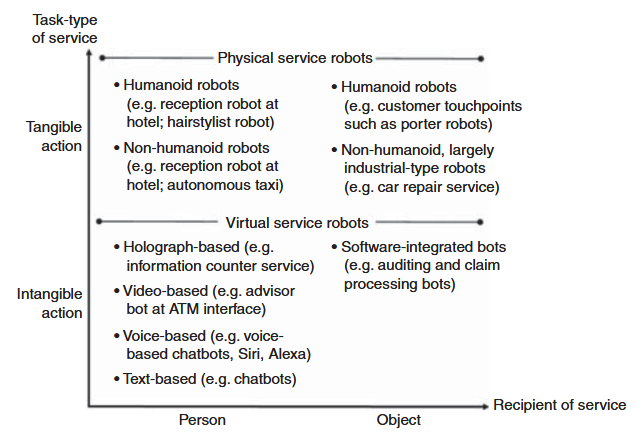
\includegraphics[width=.8\linewidth]{serviceBots.png}
        \caption{Service robots categorization by task-type and recipient of service \autocite{wirtz_brave_2018}.}
        \label{fig:serviceBots}
    \end{figure}

    Today, AI is still a constantly evolving field that is seeing bleeding-edge developments on a 
    highly frequent basis, and more recently, is becoming instrumental in many people's work and private lives 
    with the introduction of large language models (LLMs) \autocite{AIDigitalAssistants}.
    However, when developing a project that utilises AI, it is important that 
    they are ethical and human-centred in the development process, which is known as Human-Centred AI (HCAI). 
    Another issue is the "black-box problem" - the inability to know an AI's reasoning, meaning that 
    eXplainable AI (XAI) is a growing necessity \autocite{miro-nicolau_comprehensive_2025}. In focusing on 
    HCAI and XAI, the focus shifts from the machine executing the algorithms, and instead to the user and their experience 
    using the AI \autocite{AIEthics}. In his article, Shneiderman strongly advocates for the 
    promotion of HCAI for the benefit of both companies and their users, which is a commonly accepted 
    idea due to the ethical risks of using AI. Because AI calculates outcomes from its training data rather 
    than understanding social norms and perspectives, the use of it in sociotechnical systems poses serious risks 
    due to the 'traps' it can fall into, because it cannot account for every possibility such as the personal tendencies 
    and biases of its users \autocite{selbst_fairness_2019}, and therefore developers require a shift in focus - from the final product
    at the end of development to the development process itself and end users, which also echoes Shneiderman's views. 

    \subsection{Chatbots / Digital assistants}
    \begin{tcolorbox}[colback=red!5!white,colframe=orange!75!black,title=Uncertainty]
        This theme overlaps too heavily with NLP and LLMs to really be its own theme, as it would just be a repetition
        of what is said in those sections. However, it is undeniably a core aspect of this project, so I'm not sure what 
        to do for it.
    \end{tcolorbox}

    \pagebreak 
    \subsection{Natural language processing (NLP)}
    % \begin{tcolorbox}[colback=blue!5!white,colframe=blue!75!black,title=Will be rewritten in final]
    %     I'm somewhat happy with what I've written here, though I plan to go back and talk about more technical developments
    %     in NLP over time, such as Word2Vec and Seq2Seq.
    % \end{tcolorbox}

    \begin{tcolorbox}[colback=red!5!white,colframe=orange!75!black,title=Rewrite section]
        This section may need an entire rewrite. You've referred to "training data", but that isn't NLP, that's LLMs.
    \end{tcolorbox}


    The ability for a computer to interpret and understand human language greatly enhances the scale of their capabilities. This was 
    recognised during the 1950s, where machine translation from Russian to English was demonstrated for the first time, albeit in a basic form \autocite{zampolli_natural_1994}.
    NLP has become an extremely popular topic in recent years, and its applications have become very wide in scope with modern processing power, 
    performing tasks such as sentiment analysis, which is the classification of the intent of a sentence, whether positive or negative for
    example, using recent developments in AI such as recurrent neural networks (RNNs) via libraries like TensorFlow \autocite{abadi_tensorflow_2016}. To do so, 
    the training data required is immense, and often harvested from social media due to it being one of the largest repositories of 
    opinionated text data \autocite{wang_fine-grained_2016}, such as posts on platforms like Facebook and X. Another use of NLP, as previously 
    mentioned in a rudimentary form in the 1950s, is language translation. Back then, there were very limited technical options compared to 
    those that exist today, and with today's RNNs, translation can be extremely accurate, albeit more computationally intensive. 
    Both of these applications use RNNs, which are neural networks that are often superior to their alternatives such as convolutional (CNNs)
    and feedforward neural networks (FNNs) for text analysis due to the fact that they can retain information in their internal memory, which can allow them 
    to recall context, allowing them to determine the linguistic relations between sentences within a document \autocite{tang_document_2015} 
    which is especially useful in conversational interfaces where the user may say "it" to contextually refer to a previous noun from their last prompt.

    \subsection{Large language models}
    LLMs are colossal machine learning models that leverage NLP to generate text. They are currently used widely across 
    an assortment of industries in place of technical support and human resources systems, and can be supplied with text 
    prompts from users which will cause the LLM to generate a response. The system architecture of LLMs has long been a point 
    of contention due to the sheer processing power required to run them, requiring more than 8 top-range server-grade GPUs to run some of the 
    most powerful high-parameter open-source models like LLaMA 3.1 405B \autocite{dubey_llama_2024}.


    Talk about \autocite{vaswani_attention_2017} here. It's a key paper and was the foundation
    of GPT (I think). Pivot into RAG, as you're not training your own LLM due to lack of processing power. Decide between Gemini or OpenAI.
    IIRC Gemini will be far cheaper, possibly free.
    \subsection{User experience}
    I don't think I've got any papers relating to this yet.


    \subsection{Theory}

    AAAA
    
    \section{Summary}

    
    \begin{landscape}

    \chapter{Appendix}
    
    \begin{tcolorbox}[colback=red!5!white,colframe=red!75!black,title=Copied from proposal]
        This is still subject to change pending the grade from my proposal. 
        \textbf{It also needs to be updated to reflect that the proposal is now done and lit review is in progress.}
    \end{tcolorbox}

    \section{Gantt Chart}



    \begin{figure}[H]
        \centering
        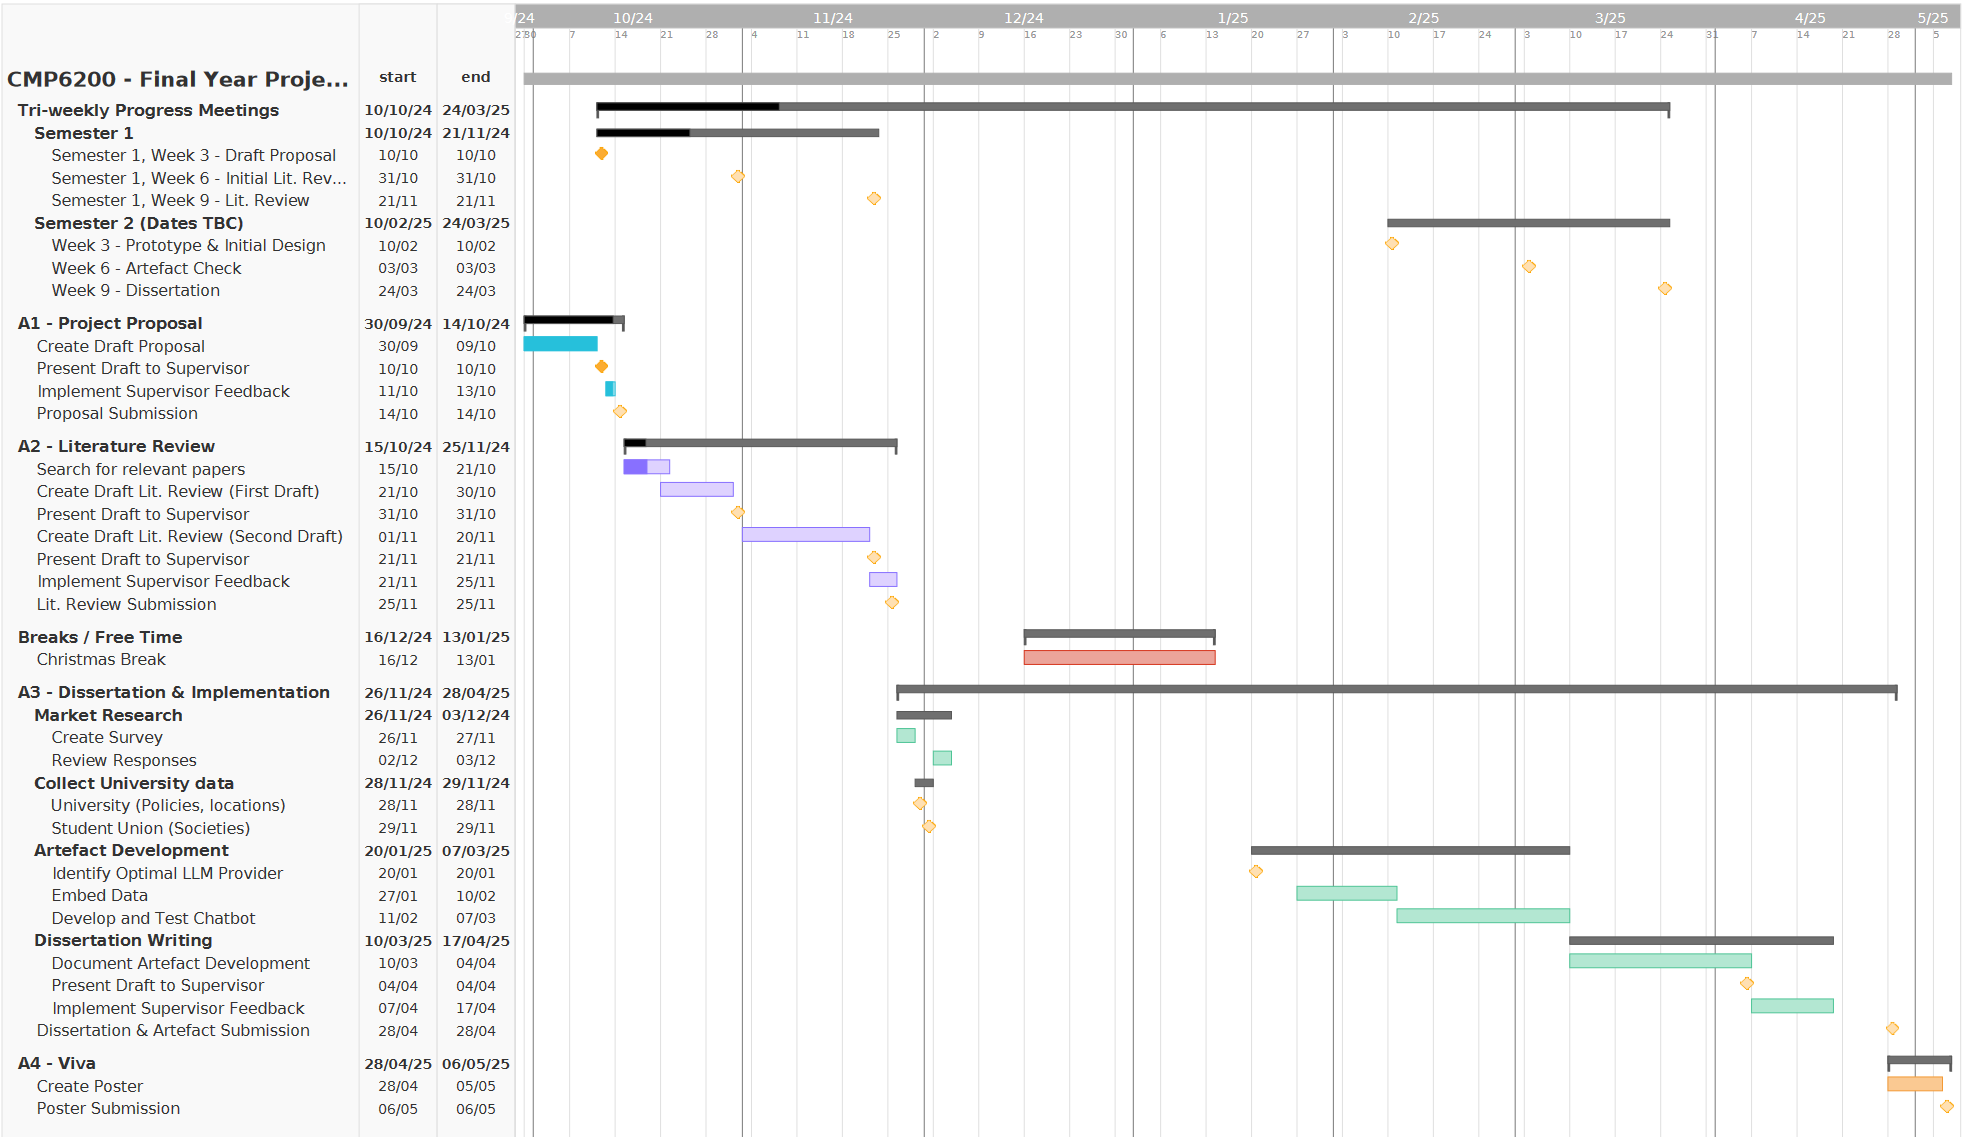
\includegraphics[width=.75\linewidth]{ProposalGantt.png}
        \caption{A conceptual Gantt chart of a development timeline.}
        \label{fig:gantt}
    \end{figure}

    \end{landscape}

    \printbibliography[keyword={refs}, title = {References}]
    \addcontentsline{toc}{chapter}{References}

    % Invisible citing sources so that they get printed here
    \nocite{IBMAIDef}
    \nocite{ICOAIDef}
    \nocite{IBMGenAI}
    \nocite{MITGenAI}
    \nocite{CloudflareLLM}
    \nocite{IBMNLP}

    \printbibliography[keyword={bib}] % Will show an error until you cite an actual "bib" source.
    \addcontentsline{toc}{chapter}{Bibliography}

\end{document}